\documentclass[master=cws,masteroption=se,english,a4paper]{kulemt}
\setup{
	title={A comparative study of cross-platform tools for mobile application development},
  	author={Michiel~Staessen},
  	assessor={ir.\ Gonzalo~Parra \and prof.\,dr.\,ir.\ Danny~Hughes},
  	promotor={prof.\,dr.\,ir.\ Erik~Duval},
  	assistant={ir.\ Gonzalo~Parra}
}

% The following \setup may be removed entirely if no filing card is wanted
\setup{
	filingcard,
	translatedtitle="Een vergelijkende studie van cross-platform tools voor het ontwikkelen van mobiele applicaties",
	udc=681.3,
	shortabstract={
		Developing mobile applications (or apps for short) that support multiple platforms is an expensive and time consuming process. Therefore, many companies are seeking refuge in cross-platform tools (CPT's) for the development of their apps. In cooperation with CapGemini, this thesis presents a comparison of two such cross-platform tools: Apache Cordova or Adobe PhoneGap and Motorola Rhodes. Both tools are compared with each other and with the native development toolkits. The comparison is based on a proof-of-concept application which should work on both smartphones and tablets with respect to both iOS and Android.
	}
}

% Uncomment the next line for generating the cover page
%\setup{coverpageonly}
% Uncomment the next \setup to generate only the first pages (e.g., if you
% are a Word user.
%\setup{frontpagesonly}

% Choose the main text font (e.g., Latin Modern)
\setup{
	font=utopia
}

%% Additional formatting settings
%  Use the chapter and headings styles as well as the ToC formatting
%  as defined in the kulemtx document style
\usepackage{kulemtx}
\headstyles{kulemtman}
\kulemtmanToC

% If you want to include other LaTeX packages, do it here.
% Finally the hyperref package is used for pdf files.
% This can be commented out for printed versions.
\usepackage[pdfusetitle,colorlinks,plainpages=false]{hyperref}
\usepackage[backend=biber,style=ieee,natbib=true]{biblatex}
\addbibresource{references.bib}
\usepackage{csquotes}
\usepackage{url}
\usepackage{amsmath}
\usepackage{amsfonts}
\usepackage{xfrac}
\usepackage{parskip}
\usepackage{pstricks}
\usepackage{pst-node}
\usepackage{pst-tree}
\usepackage{pst-plot}
\usepackage{pdfpages}
\usepackage{longtable}
\usepackage{rotating}

% Paragraph definition
\setlength{\parindent}{0pt}
\setlength{\parskip}{2.3ex plus 0.3ex minus 0.3ex}

\newcommand{\citeGartner}{\cite{Gartner:08Q2, Gartner:08Q3, Gartner:08Q4, Gartner:10Q1, Gartner:10Q2, Gartner:10Q3, Gartner:10Q4, Gartner:11Q1, Gartner:11Q2, Gartner:11Q3, Gartner:11Q4, Gartner:12Q1, Gartner:12Q2, Gartner:12Q3, Gartner:12Q4, Gartner:13Q1}}
\newcommand{\citeGartnerTab}{\cite{Gartner:11tab,Gartner:12tab}}
\renewcommand{\vec}[1]{\mathbf{#1}}
\newcommand{\html}[1]{{\small \texttt{#1}}}
\newcommand{\lsfrac}[2]{{\large $\sfrac{#1}{#2}$}}
\newcommand{\tick}{\checkmark}

\begin{document}

\begin{preface}
    Wow, it's done. It really is... I did it! But I could not have done it without the help and support of some people that I would like to thank explicitly.
    
    First and foremost, I would like to thank my promotor, professor \mbox{Erik~Duval}, for giving me the opportunity to write this dissertation. I would also like to thank my mentor, \mbox{Gonzalo Parra}, with whom I got a meeting almost every week to discuss the progress of this thesis. Thank you for your guidance and support, it was really helpful. Our contacts at Capgemini, \mbox{Jan~Verhulst} and \mbox{Jannik~Persoons}, also deserve a lot of gratitude for providing the subject and context. To my thesis colleagues, \mbox{Bert~Outtier}, \mbox{Sander~Van~Loock}, \mbox{Tim~Ameye}, and other people in the department, I would like to say thank you for sharing and giving feedback.
    
    A big thanks goes out to my family as well, and my parents in particular. Thank you for your support, for having faith, and for sponsoring my education. It really means a lot to me. Thank you, brother and sister, for showing interest in my work and thank you, Freek, for your feedback after reading my drafts and for borrowing me your old iPhone.
    
    And last --- but definitely not least --- I would also like to thank my loving girlfriend, \mbox{Charlotte~D'Haenens}. It has been a tough year for both of us but you were always there to support me, to read my drafts, to cook delicious meals even when it was my turn, \ldots\  You are truly amazing, and I love you for that!
\end{preface}

\tableofcontents*

\begin{abstract}
    Developing mobile applications (or apps) that support multiple platforms is an expensive and time consuming process. Therefore, many companies are seeking refuge in cross-platform tools (CPT's) for the development of their apps. 
    
    This thesis presents a methodology for evaluating and selecting cross-platform tools (CPT's) in a business environment and also presents the results after applying this methodology to the native development toolkits and two cross-platform tools: Apache Cordova or Adobe PhoneGap and Motorola Rhodes. 
    
    The methodology is based on a generic software selection framework and comprises of six steps. The evaluation is partly based on documentation and partly based on the implementation of a proof-of-concept application in a business context. The tools are evaluated using the analytic hierarchy process. The relative importance of the evaluation criteria are defined by Capgemini employees (a developer and an architect). The results of the evaluation reveal that, at this moment, Apache Cordova and the native development toolkits have a similar ratio of costs and benefits. However, if a third platform has to be supported some time, Cordova applications will have a better benefit-cost ratio, provided that some benefits of native development can be dropped. 
\end{abstract}

% A list of figures and tables is optional
%\listoffigures
%\listoftables

% If you only have a few figures and tables you can use the following instead
%\listoffiguresandtables

\chapter{List of Abbreviations}
\begin{flushleft}
  \renewcommand{\arraystretch}{1.1}
  \begin{tabularx}{\textwidth}{@{}p{12mm}X@{}}
    ADB & Android Debug Bridge \\
    AHP & Analytic Hierarchy Process \\
    AJAX & Asynchronous JavaScript And XML \\
    API & Application Programming Interface \\
    ASF & Apache Software Foundation \\
    B2B & Business-to-Business \\
    B2C & Business-to-Consumer \\
    CPT   & Cross-Platform Tool \\
    CRM & Customer Relationship Management \\
    CSS & Cascading StyleSheets \\
    DDoS & Distributed Denial of Service \\
    DOM & Document Object Model \\
    ERP & Enterprise Resource Planning \\
    GPS & Global Positioning System \\
    HTML & HyperText Markup Language \\
    IDE & Integrated Development Environment \\
    L\&F & Look \& Feel \\
    MCDM & Multi-Criteria Decision Making \\
    MVC & Model-View-Controller \\
    NFC & Near Field Communication \\
    SDK & Software Development Kit
  \end{tabularx}
\end{flushleft}

% Now comes the main text
\mainmatter

\chapter{Introduction}
\label{cha:intro}

The mobile industry is without a doubt one of the most vibrant industries at the moment. It is characterized by rapid growth and intense competition which has led to fragmentation. This chapter first presents an overview of the evolution in the mobile device landscape, then explains the problem of fragmentation and how cross-platform tools (CPT's) can help solve this problem and finally, the goals of this thesis are defined.

\section{The mobile device landscape}

Mobile phones have been around since the nineties but ever since the (nearly simultaneous) introduction of the iPhone 3G and the HTC Dream in 2008, smartphones are taking over from traditional cell phones or feature phones. A feature phone (sometimes also called a dumb phone) is a low-end mobile phone, providing only basic telephony and texting capabilities. Smartphones on the other hand are high-end devices that combine the functionality of mobile phones with the functionality of a portable computer. These devices have advanced computing power and often include multiple connectivity options (cellular, Wi-Fi, Bluetooth, NFC, etc.), sensors (GPS, compass, accelerometer, etc.), applications, etc. In the last five years, smartphone sales have grown tremendously. According to quarterly studies by Gartner\footnote{Gartner is an American research and advisory firm, specialized in information technology, \url{http://www.gartner.com}.} \citeGartner, smartphone sales have grown 544\% since the second quarter of 2008 (see \fref{fig:smartphone-sales}). Smartphones are becoming ubiquitous and in some regions like the United States, smartphone penetration\footnote{this is the ratio between smartphones and all mobile phones} has already reached more than 50\% \cite{Nielsen:2012}. 

\begin{figure}[h]
    \centering
    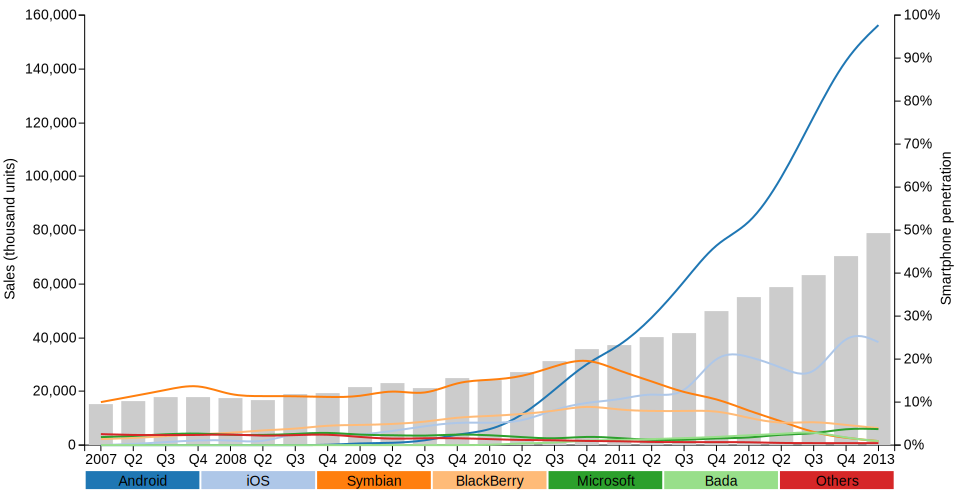
\includegraphics[width=\textwidth]{../resources/figs/smartphone_sales.pdf}
    	\caption{Evolution of worldwide smartphone sales by operating system (lines) and smartphone penetration (bars). Source: Gartner \citeGartner}
    	\label{fig:smartphone-sales}
\end{figure}

Each of these smartphones comes with a mobile operating system which allows owners to run third-party software, typically called applications or apps for short, on their device. These applications play an important role as they drive the network effects associated with a certain platform. Applications create additional value for a platform, which attracts new users. Whenever a platform attracts more users, it becomes even more valuable. This vicious circle is called a network effect. Network effects make it hard for new platforms to gain traction which is visible in \fref{fig:smartphone-sales} and \fref{fig:smartphone-share}. Android and iOS are currently dominant (and continue growing) while other platforms are either in decline (like Symbian and Blackberry, formerly RIM) or have a hard time getting traction (like Windows Phone, the successor of Windows Mobile, which already existed long before Android and iOS).

\begin{figure}[h]
    \centering
    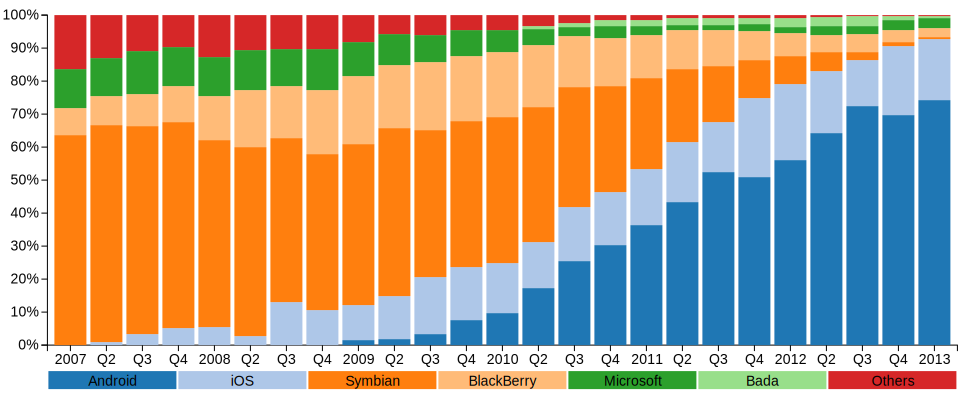
\includegraphics[width=\textwidth]{../resources/figs/smartphone_share.pdf}
    \caption{Evolution of worldwide smartphone market share by operating system.\newline Source: Gartner \citeGartner}
    \label{fig:smartphone-share}
\end{figure}

However, there is no single major platform. In addition, the IDC\footnote{International Data Corporation is another American research, analysis and advisory firm, specializing in information technology, telecommunications and consumer technology, \url{http://www.idc.com}.} predicts that Windows Phone will gain a significant market share by 2016 and that 90\% of the worldwide smartphone market will then be covered by Android, iOS and Windows Phone \cite{IDC:phone}. Hence, it is reasonable to assume that there will always be more than one major platform.

The second type of mobile devices are tablet computers or tablets. In their current form, tablets are somewhat similar to smartphones but they have larger touchscreens (customarily starting at 7 inches in diagonal) and do not offer basic telephony. However, some of them do have a cellular radio that can be used for data transmission. Because of their hardware similarities, their software is also similar: the dominant smartphone operating systems are also used in tablets.

As with smartphones, tablets gained a lot of popularity since the launch of the iPad and Android tablets. According to other studies by both Gartner \citep{Gartner:11tab,Gartner:12tab} and the IDC \citep{IDC:tablet}, tablets will continue to gain popularity and sales will be mainly driven by iPads and Android tablets (see \fref{fig:tablet}). Even though these studies disagree on which operating system will be used in most devices, they both predict there will be three major platforms: iOS, Android and Windows. 

\begin{figure}[h]
    \centering
    \includegraphics[width=\textwidth]{../resources/figs/tablet_sales.pdf}
    \caption{Prediction of worldwide tablet sales and market share.\newline Source: Gartner \citeGartnerTab}
    \label{fig:tablet}
\end{figure}

\section{The problem of fragmentation}

Fragmentation can be defined as the fact that all devices are different; there is no uniform device. This is called device fragmentation. In fact, all mobile devices can be divided into multiple, overlapping categories like operating system or platform (called platform fragmentation), operating system version or runtime (called runtime fragmentation), screen size and screen resolution (called screen fragmentation) and many more. Hence, fragmentation is a multi-dimensional problem. 

Fragmentation is generally beneficial for consumers, carriers and manufacturers. The more different devices there are, the more likely a consumer is to find a device that fits his needs. For developers on the other hand, fragmentation is usually disadvantageous. It forces them to test their applications on multiple devices to guarantee the desired user experience. This is expensive and time-consuming. 

The nature of a platform strongly influences the fragmentation issues within said platform. For instance, Apple can manage fragmentation issues pretty well because iOS is a closed platform and the only devices running iOS, called iDevices, are designed by Apple itself. In fact, these devices show many similarities. Android on the other hand is an open system. Android is being developed privately at Google, but the source code of every release is publicly available under the Apache 2.0 License, which means that everybody is allowed to customize it. The ability for manufacturers to alter the operating system has largely contributed to the success of Android. 

Mobile device manufacturers are eager to modify the Android operating system to differentiate their product from their competitors. As such, they create their own Android flavour, i.e. a distribution of Android with a custom user interface (like HTC Sense, Samsung TouchWiz, etc.), custom software, additional market places, etc. However, applying these modifications over and over for every new release of Android is cumbersome and costly which is why device manufacturers do not often provide updates for their devices. This has led to the notorious Android runtime fragmentation, which is depicted in \fref{fig:android_runtimes}. The adoption rate for new versions is low and is caused by the nature of Android. Developers have to support multiple versions, which is tedious. 

\begin{figure}[h]
    \centering
    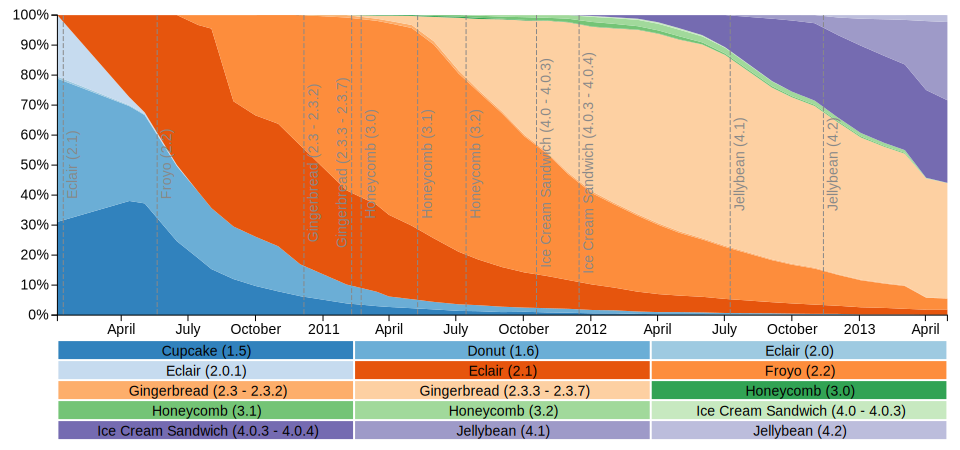
\includegraphics[width=\textwidth]{../resources/figs/android_runtimes.pdf}
    \caption{Historical Android runtime fragmentation. The data for this graph was aggregated from \cite{Android:Versions} using the Internet Archive (\url{http://archive.org}).}
    \label{fig:android_runtimes}
\end{figure}

Unlike Google, Apple does not publicize runtime statistics but developers \cite{Smith:2013} and online advertisers \cite{Chitika:2013} can confirm fast adoption rates for iOS. On iOS, developers can make use of new functionality much faster. However, as Apple starts to drop support for some of its devices that are still in use (like for instance the original iPad and the iPod third generation), it introduces runtime fragmentation. Because of this, iOS developers will have to support the latest two versions of iOS.

Android and iOS are used in both smartphones and tablets. There are only few different iDevices  but in contrast, there is an enormous number of Android devices. At the time of writing, the Google Play Store\footnote{Google Play is the official marketplace for Android applications.} supports 2935 different device configurations, distributed across 63 manufacturers. All these devices come  with varying screen sizes and resolutions which implies that applications also have to deal with this. On Android, this is solved by a flexible layout system. On iOS, this is solved by centering the user interface in the middle of the screen. For instance, applications that are not optimized for the 4-inch display of the iPhone 5 (or iPod Touch, 5th generation) will have black bars on the top and the bottom. High-density displays\footnote{A high-density display has about twice the pixel density of a regular display.}, like the Retina display, do not really introduce a new screen resolution because every logical pixel is represented by four physical pixels and this conversion is mostly handled by the operating system.

There are still a lot more dimensions to the fragmentation problem like computing power, available sensors, available networking, etc. but these differences can be categorized under device fragmentation. In conclusion, fragmentation among Android devices is rather high compared to iDevices.

\section{Cross-platform tools to the rescue}

In the current economy, information is a company's most valuable asset and the rate at which information exchange takes place increases every day. Mobile Internet-enabled devices are a valuable resource for this purpose and, as a consequence, many companies want mobile applications for their businesses. However, in an ever-changing and unpredictable industry like the mobile industry, it is unwise to target a single platform. This could eventually lead to vendor lock-in, i.e. all operations (or a significant part thereof) are built on equipment or software of a single vendor which puts that vendor in a bargaining position. Companies will try to avoid these situations at all costs and they will do so by asking for cross-platform solutions. 

Making a solution work across platforms typically requires that the software has to be implemented multiple times: one time for each platform. This is costly and time-consuming. Cross-platform tools (CPT's) can help to solve this problem because they allow to support multiple platforms from a single codebase. Hence, they lower entry barriers (access to new platforms) and exit barriers (lock-in) \cite{VMCPT:2012}. 

Cross-platform tools try to solve three major problems \cite{VMCPT:2012}: 

\begin{enumerate}
    \item \textbf{Fragmentation} Fragmentation issues, as described above, are a struggle for every developer. They are forced to test their applications on a large number of devices in order to be able to guarantee the desired user experience. A cross-platform tool can help to identify platform quirks and provide workarounds. 
    \item \textbf{Access to new platforms} Targeting a new platform is generally hard. Developers have to learn yet another SDK and/or programming language in order to deliver applications for this platform. A cross-platform tool can make abstraction of platform differences which allows developers to reuse their current skills. This drastically reduces the effort that is needed to target a new platform. Bear in mind that a new platform does not necessarily have to be a smartphone or tablet operating system, it could also be the operating system of a television set, or a car console, etc.
    \item \textbf{Development inefficiency} Maintaining codebases for multiple platforms is a difficult and costly task. When a new feature is introduced, it has to be applied to all codebases. With the use of a cross-platform tool, all code is contained within a single codebase and no time is lost while synchronizing features and executing other maintenance tasks across codebases. This reduces cost while increasing productivity. 
\end{enumerate}

\section{Goals}

It is clear that there is a large demand for cross-platform solutions and that there are a lot of benefits associated with the use of cross-platform tools. Therefore, this thesis will try to identify a suitable cross-platform tool for mobile application development. This is a two-step process. First, a methodology will be defined for evaluating and selecting cross-platform tools. Second, this methodology will be used to evaluate two cross-platform tools (Apache Cordova and Motorola Rhodes) and the native SDK's in a business environment, provided by Capgemini\footnote{Capgemini is a multinational IT consulting company, \url{http://www.capgemini.com}.}. From this evaluation, the best-suited alternative will be selected. 
\chapter{Literature Study}
\label{chap:literature}

% TODO: write introductory text
\TODO{write introductory text}

\section{Multi-Criteria Decision Making (MCDM)}
\label{sec:mcdm}

Finding the right software package is often a daunting task. In order to suit the end-user's needs, the software should meet a large number of -- sometimes conflicting -- requirements and will result in making important trade-offs. Because of the these characteristics, software selection can be modeled as a Multiple-Criteria Decision Making (MCDM) problem \cite{Jadhav:2009, Jadhav:2011}.

There are two categories of MCDM problems: Multiple-Attribute Decision Making (MADM) problems and Multi-Objective Decision Making (MODM) problems. The first category involves sorting and ranking of a limited number of available alternatives, based on a number of decision criteria. In the latter category, there are no alternatives specified beforehand and the number of alternatives is effectively infinite \cite{Kahraman:2008}. 

The software selection process belongs to the category of MADM problems. Their goal is to find the best alternative in a set of alternatives and at the same to time create a ranking of all these available alternatives. % TODO: Reference!

There are a plethora of solution methods for the MADM problem. The following subsections will describe the most frequently used methods in literature, together with their advantages and disadvantages. 

% TODO: discuss cost vs benefit
\TODO{General remark for all methods: Separate costs from benefits, allowing to make a cost-benefit analysis afterwards. }

\subsection{Arbitrary scoring models} 
% TODO RFC: Is this a good naming?
\TODO{Question: Is this an appropriate name?}

There are a number of arbitrary scoring models but they all have one thing in common: for each criterion, the values are translated to a numerical score. In some cases, this score can be derived from the value of the criterion itself (e.g. speed, age, cost, \ldots). In other cases, a mapping is provided (e.g. in order to obtain a score $s$, at least features $f_1$, $f_2$ and $f_3$ should be supported).

Different methods are available to select potential candidates using these scores \cite{Kahraman:2008}:

\begin{itemize}
    \item When the ``dominance'' method is used, one alternative should clearly outperforms the other alternatives for at least one criterion. 
    \item When the ``maximin'' method is used, the final score of each alternative is equal to the lowest score of all criteria for this alternative.
    \item When the ``maximax'' method is used, the final score of each alternative is equal to the highest score of all criteria for this alternative.
    \item When the ``conjunctive'' method is used, an alternative should exceed certain thresholds for \emph{all} criteria.
    \item When the ``disjunctive'' method is used, an alternative should exceed certain thresholds for \emph{at least one} criterion. 
\end{itemize}

Additionally, the importance of the criteria can be accounted for by assigning weights. The final score can be calculated as the weighted sum, weighted product or weighted average.

The strength of these methods is that they are the most easy to use. However,  scores and weights are assigned arbitrarily and might get tough when there are a lot of criteria. Also, not all criteria are suitable for conversion into a numerical scale \cite{Jadhav:2009}.

\subsection{Analytic Hierarchy Process (AHP)}
\label{sec:ahp}

The Analytic Hierarchy Process (AHP) is ``a multi-criteria decision making approach in which factors are arranged in a hierarchic structure'' \cite{Saaty:1990}. It is developed by Thomas L. Saaty and is based on pairwise comparisons of both criteria and alternatives. 

The strengths of the AHP are that it (1) enables decision makers to structure a problem into a hierarchy, (2) that is provides a powerful tool for handling both quantitative and qualitative multi-criteria decision making problems and (3) that this system can deal with inconsistency \cite{Jadhav:2009}. 

The analytic hierarchy process consists of three stages. In the first stage, the factors that are important for the decision are organized into ``a hierarchic structure descending from an overall goal to criteria, subcriteria and alternatives in successive levels''. Organizing the factors in such structure helps the decision maker in getting an overview of the potentially complex relationships and also helps to assess the relative importance of the issues in each level. 

Structuring information in a tree is also backed by experiments of psychologist George Miller. He found that people can only deal with a few facts simultaneously; more precisely, seven plus or minus two \cite{Miller:1956}. 

In the second stage, the analytic hierarchy process establishes a ranking of the alternatives based on paired comparisons. 

\TODO{connect paragraphs}

Consider the case in which the relative comparison is derived from a given scale. For instance, where you have $n$ stones $A_1, \ldots, A_n$ with weights $w_1, \ldots, w_n$ respectively. 

\begin{gather}
    \begin{bmatrix}
        w_1/w_1 & w_1/w_2 & \ldots & w_1/w_n \\
        w_2/w_1 & w_2/w_2 & \ldots & w_2/w_n \\
        \vdots  & \vdots  &        & \vdots  \\
        w_n/w_1 & w_n/w_2 & \ldots & w_n/w_n    
    \end{bmatrix} % 
    \begin{bmatrix}
        w_1    \\
        w_2    \\
        \vdots \\
        w_n
    \end{bmatrix} = %
    n %
    \begin{bmatrix}
        w_1    \\
        w_2    \\
        \vdots \\
        w_n
    \end{bmatrix} \Longleftrightarrow %
    Aw = nw
    \label{eq:ahp}
\end{gather}

If $n$ is an eigenvalue of $A$, then $w$ is the corresponding eigenvector. The trace of a matrix, the sum of the elements on the main diagonal, is equal to the sum of its eigenvalues. Matrix $A$ has rank one because all rows of $A$ are linearly dependent on the first row and consequently, all eigenvalues except one are zero. Hence, $tr(A) = n$ and $n$ is the largest or pricipal eigenvalue of $A$.

\TODO{Prove validity of eigenvector method in AHP using \cite{Sekitani:1999, Saaty:2003}?}

\TODO{Add example}

The weakness of AHP is that it is a time consuming method due to the large number of pair-wise comparisons. Also, the ordering may change entirely when other alternatives are taken into account.

\subsection{Fuzzy MCDM}
\label{sec:fuzzy}

% TODO: Write section
\TODO{Write section}

Fuzzy logic was introduced in the mid `60s by Zadeh and was later applied to MCDM problems in the late `70s. Fuzzy logic allows to reason with imprecisely specified criteria like very high performance, low performance, etc. In classical approaches like those described above imprecision is dealt with first. When using the fuzzy approach, these imprecisions are only dealt with in the end, and only if necessary.

Fuzzy MCDM is based on three concepts \cite{FuzzySetApproach}:

\begin{enumerate}
    \item The set of alternatives is a \emph{fuzzy set}, i.e. the alternatives aren't precisely defined. The decision will thus be taken in a \emph{fuzzy environment}. 
    \item The decision is based on an aggregation of fuzzy preferences among alternatives.
    \item The decision is based on an evaluation of alternatives using a linguistic description.
\end{enumerate}

More concrete, let $A = \{a_1, \ldots, a_n\}$ be a finite set of given alternatives and let there be $m$ imprecisely defined criteria. Every alternative fulfills a criterion in a certain degree or does not fulfill it at all. In other words, for each criterion $G_j, j = 1, \ldots, m$ there is a set $G_j \subset A$ containing the alternatives fulfilling the criterion and the degree in which an alternative $a_i$ fulfills $G_j$ is expressed by the membership degree $G_j(a_i)$.

In order to decide the MCDM problem, constraints must be defined for each criterion. These constraints are specified as fuzzy sets as well meaning that a constraint $C_j$ is associated with a set $C_j \subset A$ containing the alternatives fulfilling $C_j$ in a certain degree. Again, a membership degree $C_j(a_i)$ is given.

Consequently, there are two fuzzy sets for every $j, j = 1, \ldots, m$, namely $G_j$ and $C_j$. The decision can now be obtained by composition and is given by the fuzzy set 
\begin{equation}
    D = (G_1 \alpha C_1) \beta \ldots \beta (G_m \alpha C_m)
\end{equation}
where $\alpha$ and $\beta$ are suitable fuzzy set operations. The alternative $a_k$ with the highest membership degree $D(a_k)$ is the best alternative.

\TODO{paraphrazed same source in previous three paragraphs, need a reference on each?}

\TODO{Add an example: For example, when buying a house these criteria could be \emph{nice neighbourhood}, \emph{great parking facilities}, \emph{reasonable price}, etc.}



\section{Software evaluation methodology}
\label{sec:selection_method}

Based on their literature review \cite{Jadhav:2009}, the authors have proposed a generic, six-stage methodology for the selection of software packages \cite{Jadhav:2011}.

\begin{enumerate}
    \item \textbf{Define selection criteria.} In the first stage, the evaluator defines the essential requirements for the software. If a certain software package does not meet a selection criterion, it is not a considered to be a suitable candidate and it should not be considered for further evaluation. 
    \item \textbf{Identify potential candidates.} During the next step, the evaluator searches for potential candidates. This step will result in a list of potential candidates.
    \item \textbf{List selected alternatives.} In this step, the evaluator will use the requirements from stage 1 to filter the list obtained from the previous stage. 
    \item \textbf{Define evaluation criteria.} In this stage, the evaluator has to define the evaluation criteria, arrange them in a hierarchy and define the value scales for each criterion. 
    \item \textbf{Evaluate selected alternatives.} During this phase, the evaluator will make a detailed comparison of the alternatives using the criteria obtained from the previous stage. A methodology like AHP can be used in this stage.
    \item \textbf{Select the most suitable alternative.} In this final step, all alternatives are ranked using the comparison results from the previous stage. Now, the best alternative can be chosen from the list of candidates. In general, a number of software packages will be taken into consideration and a selection will be made after additional steps (like for instance a cost-benefit analysis and/or contract negotiations with the vendor). 
\end{enumerate}

In the original paper \cite{Jadhav:2009}, the authors also suggest to include an additional evaluation stage after the selected packages has been implemented and integrated. During that stage, one should verify that the selected package does indeed meet the requirements.

\section{Mobile Architectures}

% TODO: talk about mobile hub
\TODO{Explain Mobile Hub/Mobile Orchestrator}

% TODO: discuss cost for each architecture
\TODO{discuss cost for each architecture}

There are already a number of paradigms for cross platform mobile application development \citep{Friese}. This section presents an overview of the available strategies by comparing different aspects: performance, look and feel, platform access, programming languages, development cost and distribution.

\subsection{Native App}

A native app is an application that is specifically designed to run on a particular platform. It is the default approach to develop applications for mobile devices. \fref{fig:native} shows an illustration of the overall architecture of such an app. 

\begin{figure}[h!]
    \begin{center}
        \includegraphics[width=\textwidth]{figs/native.pdf}
        \caption{
            Overall architecture of a native app. 
        }
        \label{fig:native}
    \end{center}
\end{figure}

Native apps are developed with the supplied SDK. Developers will need to get acquainted with the programming language used by said SDK but in return they will get full access to the platform and its features. As a result, the best performance can be obtained with this kind of app.

For the user interface, developers can use lots of interface elements such that they can present a familiar look and feel to the end user. 

Native apps can be easily distributed through an online marketplace like for instance the App Store or Google Play. 

Because native apps are designed to run on one platform only, this development strategy is not very well suited for cross platform development. If an application should run on multiple platforms, it has to be developed for each platform separately. This is costly.

\subsection{Web App}

Web apps are websites that are optimized for mobile browsers. Since every platform comes with a browser, this is the easiest way to get an application running on all platforms. An overview of the overall architecture for this kind of app is given in \fref{fig:web}.

\begin{figure}[h!]
    \begin{center}
        \includegraphics[width=\textwidth]{figs/web.pdf}
        \caption{
            Overall architecture of a web app.
        }
        \label{fig:web}
    \end{center}
\end{figure}

Web apps are not nearly as powerful as native apps. First of all, the application is not stored on the device. Web apps require an active internet connection which cannot always be guaranteed. Second, they are built with web technologies like HTML, CSS and JavaScript, which have to be interpreted by the browser at runtime. Third, web apps cannot access the system which means they cannot make use of the many unique features of a mobile device. 

With HTML5, web apps can get more powerful. They will be able to access device features, like the camera and other sensors \cite{MobileHTML5}. They will not even require an active internet connection because they can be cached on the device. However, HTML5 is still a draft and a lot of mobile browsers lack proper HTML5 support.

From a user interface perspective, web apps can be a problem as well. 
% TODO: complete paragraph
\TODO{complete paragraph}

Web apps are distributed easily: the only requirement is a valid URL. Web apps cannot be installed on the device though, but there are workarounds using Web Clips on iOS \cite{Safari:webclips} and bookmarks on Android. 

\subsection{Hybrid App}

Hybrid applications are the logical next step, combining native apps and web apps. The actual application is a web site, embedded in a web view, part of a native wrapper. The embedded website can access (parts of) the system through a bridge. An overview of the overall architecture is shown in \fref{fig:hybrid}. 

\begin{figure}[h!]
    \begin{center}
        \includegraphics[width=\textwidth]{figs/hybrid.pdf}
        \caption{
            Overall architecture of a hybrid app.
        }
        \label{fig:hybrid}
    \end{center}
\end{figure}

Hybrid apps are part native app, part web app. Performance will be similar to web apps but some parts can be optimized by using native code. The websites inside the hybrid app are also much more powerful because they can access many device features that aren't available in HTML(5) through the bridge.

When it comes to the user interface, hybrid apps suffer from the same problem as web apps. 

Because hybrid apps are wrapped in a native container, they can be distributed just like native applications, through online marketplaces. 

\subsection{Interpreted App}

In an interpreted app, instructions in some language are translated to native instructions at runtime. \fref{fig:interpreted} shows the overall architecture of an interpreted app.

\begin{figure}[h!]
    \begin{center}
        \includegraphics[width=\textwidth]{figs/interpreted.pdf}
        \caption{
            Overall architecture of an interpreted app.
        }
        \label{fig:interpreted}
    \end{center}
\end{figure}

Performance of interpreted apps depends on the interpreter and interpreted language but is better than web apps on average, though not as good as native apps. 

In an interpreted app, the user interface description is interpreted and rendered on the device using native interface elements. An interpreted app will have a familiar look and feel.

From the outside, interpreted apps -- just like hybrid apps -- look like native apps and can be distributed through online marketplaces.

\subsection{Cross Compiling}

Instead of translating instructions at runtime, one could translate instructions at compile time. The process is called cross compiling and the result is a truly native app. The overall architecture is sketched in \fref{fig:crosscompiled}. 

\begin{figure}[h!]
    \begin{center}
        \includegraphics[width=\textwidth]{figs/crosscompiled.pdf}
        \caption{
            Overall architecture for cross compiled apps. 
        }
        \label{fig:crosscompiled}
    \end{center}
\end{figure} 

\subsection*{Summary}

\tref{tab:architectures} summarizes the results of the discussed strategies. It is important to note that there is no universal strategy that fits all use cases. A strategy must be chosen carefully, taking into account the client's wishes.

\begin{table}[h!]
    \begin{center}
        \begin{tabular}{l|c|c|c|c|c}
                             & Native      & Web                   & Hybrid      & Interpreted & Cross Compiled\\
            \hline
            Performance      & high        & low                   & rather low  & average     & high          \\
            Platform Access  & \checkmark  & $\times$ / \checkmark & \checkmark  & \checkmark  & \checkmark    \\
            Look \& Feel     & native      & non-native            & non-native  & native      & native        \\
            Distribution     & marketplace & URL                   & marketplace & marketplace & marketplace   \\
            Development cost & high        & rather low            & average     & average     & average       \\
        \end{tabular}
		\caption{
			Summary of cross platform mobile application development strategies.
		}
		\label{tab:architectures}
    \end{center}
\end{table}

\section*{Summary}
\chapter{Methodology}
\label{chap:methodology}

Based on the insights gained from the literature, this chapter describes the research methodology used to evaluate the selected cross-platform tools. 

In \cite{jadhav:09}, the authors present a generic stage-based methodology for the selection of software packages. 

\begin{enumerate}
    \item Determine the need for purchasing the system and preliminary investigation of the availability of suitable candidates.
    \item Short candidate listing
    \item Eliminate 
\end{enumerate}


\section{Define selection criteria}

\section{Select }

\section{Define evaluation criteria}

\section{Evaluation}

\section{}



\chapter{Studied Tools}
\label{chap:tools}

\chapter{Evaluation}
\label{chap:evaluation}

\TODO{Repeat the Methodology sections, this time doing the actual comparison.}

\section{Portability}

\TODO{High-level portability score}

\subsection{Platform support}

\paragraph{Android \& iOS} \TODO{no additional platforms}

\paragraph{Apache Cordova} \TODO{For now: Windows Phone, BlackBerry. For later: Tizen, Qt, Firefox Mobile OS, Ubuntu Mobile, Windows (Desktop)}

\paragraph{Motorola Rhodes} \TODO{Windows Phone, BlackBerry}

\paragraph{Verdict} \TODO{pairwise scores in table}

\subsection{Toolset reuse}

\paragraph{Android \& iOS} \TODO{Needed: Mac computer, Xcode, Eclipse}

\paragraph{Apache Cordova} \TODO{Any operating system with a text editor or web IDE, cloud builder available}

\paragraph{Motorola Rhodes} \TODO{Any operating system with a Ruby IDE, cloud builder available}

\paragraph{Verdict} \TODO{pairwise scores in table}

\subsection{Code reuse}

\paragraph{Android \& iOS} \TODO{Absolutely nothing!}

\paragraph{Apache Cordova} \TODO{100\%, Except for native plugins: 0\%}

\paragraph{Motorola Rhodes} \TODO{Any operating system with a Ruby IDE, cloud builder available}

\paragraph{Verdict} \TODO{pairwise scores in table}

\subsection{Portability Summary?}

\TODO{summary with all portability values?}

\section{Application Experience}

\TODO{High-level Application Experience score}

\subsection{Native Integration}

\paragraph{Android \& iOS} \TODO{list native device APIs}

\paragraph{Apache Cordova} \TODO{list native device APIs}

\paragraph{Motorola Rhodes} \TODO{list native device APIs}

\paragraph{Verdict} \TODO{pairwise scores in table}

\subsection{UI Capabilities}

\paragraph{Android \& iOS} \TODO{list UI elements \& styling options}

\paragraph{Apache Cordova} \TODO{list default UI (form) elements in HTML5}

\paragraph{Motorola Rhodes} \TODO{same as Cordova minus HTML5 polyfills!}

\paragraph{Verdict} \TODO{pairwise scores in table}

\subsection{Performance}

\TODO{subjective testing allowed? AHP can make up for it?}

\paragraph{Android \& iOS} \TODO{Best}

\paragraph{Apache Cordova} \TODO{average/worse than average}

\paragraph{Motorola Rhodes} \TODO{Worst}

\paragraph{Verdict} \TODO{pairwise scores in table}

\subsection{Application Experience Summary?}

\section{Productivity}

\TODO{High-level productivity score}

\subsection{Skill reuse}

\paragraph{Android \& iOS} \TODO{Android is Java, iOS is Objective C. Java is known from EE, objective C is not. about 50\%}

\paragraph{Apache Cordova} \TODO{Cordova is HTML + JS + CSS, completely known: 100\%}

\paragraph{Motorola Rhodes} \TODO{Ruby + HTML + JS + CSS, not completely known: 40--50\%}

\paragraph{Verdict} \TODO{pairwise scores in table}

\subsection{Tooling}

\paragraph{Android \& iOS} \TODO{Great IDE for iOS, Good Eclipse plugin for Android}

\paragraph{Apache Cordova} \TODO{Few or no tools (Ripple emulator maybe?), Cloud builder?}

\paragraph{Motorola Rhodes} \TODO{Awful (out of the box), cloud builder?}

\paragraph{Verdict} \TODO{pairwise scores in table}

\subsection{Testing}

\paragraph{Android \& iOS} \TODO{}

\paragraph{Apache Cordova} \TODO{}

\paragraph{Motorola Rhodes} \TODO{}

\paragraph{Verdict} \TODO{pairwise scores in table}

\subsection{Productivity Summary?}

\section{Global verdict}

\chapter{Conclusion}
\label{chap:conclusion}

\section{Goals}
\label{sec:goals}

This thesis had two major goals. The first goal was to design a methodology to evaluate and select a cross-platform tool for mobile application development. The second goal was to use this methodology to evaluate real cross-platform tools and select the best candidate. The methodology used was inspired by the generic software package selection, presented by \citet{Jadhav:2011}, and comprises of six highly customizable stages. Each of these stages has been presented in Chapter \ref{chap:methodology}. 

During the first stage, the selection criteria were gathered. These are the most essential requirements that a cross-platform tools has to meet. The selection criteria were defined by Capgemini and require cross-platform tools to produce native applications for both Android and iOS and for both smartphones and tablets. 

Next, a list of potential candidates was composed from Internet searches and literature. An extensive list of cross-platform tools was was composed from ``Cross-platform developer tools 2012'', a report by VisionMobile on this subject \cite{VMCPT:2012} and ongoing research by research2guidance. Subsequent Internet searches did not reveal new tools.

During the third stage, this list of potential candidates was filtered using the selection criteria from the first stage and from the resulting list, two cross-platform tools were selected for evaluation. These tools are Apache Cordova and Motorola Rhodes (see Chapter \ref{chap:tools}). The native development kits for both Android and iOS were also included as a baseline for the evaluation. 

Subsequently, the evaluation criteria were defined from literature review and interviews with a developer, a mobile architect, and a salesman at Capgemini. Eleven evaluation criteria were identified: platform support, toolset reuse, code reuse, access to hardware, integration with platform-specific services, native look \& feel, user interface capabilities, performance, skill reuse, tooling, and testing. These criteria are organized into a hierarchy with because literature suggests that humans can only deal with 7 plus or minus 2 pieces of information simultaneously \cite{Miller:1956}.

During the fifth stage, the alternatives were evaluated using these evaluation criteria. For this evaluation, the analytic hierarchy process (AHP) \cite{Saaty:1980} was used. This method assigns weights to both criteria and alternatives based on judgements that originate from pairwise comparisons. In order to formulate a more reliable judgement, a proof-of-concept application was implemented with the studied tools. The relative importance of the evaluation criteria is judged by a developer and a mobile architect. Because a different ranking of the evaluation criteria could lead to a different ranking of the cross-platform tools, the evaluation covers these two perspectives separately.

During the final stage, the candidates that are most suited were carefully selected. This required a cost-benefit analysis to ascertain that the selected alternative was also cost-effective. For this cost-benefit analysis, development time was used as a cost driver and the scores for the alternatives, obtained from the evaluation, were used as benefits. From this analysis, it was concluded that Apache Cordova is currently equally cost-effective as the native development kits when only targeting Android and iOS. However, if in the future a third platform has to be supported, Cordova will be more cost-effective because the application can be completely reused on the next platform, provided that the lost benefits are acceptable.

\section{Reflection and future work}
\label{sec:reflection}

The methodology presented in this thesis ends with the selection of a cross-platform tool. However, the usefulness of this tool is never validated. Hence, a seventh, validation stage seems desirable. However, it is not possible to include this step in the timeframe of this thesis because such validation requires that the tool is used in a production environment for quite some time. The prolonged use of a particular tool in a large-scale environment will definitely reveal more benefits and/or issues than a simple proof-of-concept application can in a small-scale and controlled environment. Ergo, this seventh step is of utmost importance after the selection of a cross-platform tool.

Also, the mobile industry is rapidly evolving, which inherently makes cross-platform tools moving targets. The outcome of this study will probably be different in one year from the moment of writing. This makes continuous evaluation of the available tools a necessity and introduces a feedback loop in the evaluation process. New technologies often provide less functionality in the early stages of its life cycle but they can quickly overcome the functionality of the current technologies. New tools can be deemed ineffective at a certain time, but may become more effective than the current tools in the future. Continuous evaluation is recommended.

From the cost-benefit analysis in this study it is concluded that Apache Cordova and the native development kits are currently equally cost-effective. If a company decides to use Cordova for a number of its applications, a new problem rises because Cordova only wraps (mobile) web applications. There is a large number of tools available for (mobile) web development. Working with each of these technologies will create a different experience, both for developers and end-users, which motivates the need for another comparative study, a study that compares tools for (mobile) web development. 

During the evaluation phase, the criteria are weighted using the judgements of only two individuals. However, having multiple individuals evaluate the alternatives was simply not an option and only two employees were available for questioning. The evaluation is based on the judgement of the author. Hence, the result does not represent the animo among developers and architects but result rather represents a single case of combined judgement of three individuals. In future work, it might be wise to increase the sample size of the questioned people and evaluators in order to obtain statistically valid results. 

For the evaluation, the analytic hierarchy process is used. One of the strengths of this method is that it is based on pairwise comparison but this could also become a weakness when a large number alternatives needs to be evaluated. This problem can be solved either by using another evaluation technique or by making modifications to the AHP to deal with these numbers, as is suggested in literature.

The proof-of-concept application was used to gain the experience to formulate a more reliable judgement about the tools. The application itself has not been completed, let alone production ready. The development of the Rhodes application has even been cancelled due to the bad quality of that cross-platform tool. The Cordova application currently wraps all the necessary source code. Instead, future versions could fetch the code from a URL and cache this code using AppCache. This way, the application can be kept up-to-date without the need for updating the outer shell.





%\include{chap-2}
% ... and so on until
%\include{chap-n}
%\chapter{Conclusion}
\label{chap:conclusion}

\section{Goals}
\label{sec:goals}

This thesis had two major goals. The first goal was to design a methodology to evaluate and select a cross-platform tool for mobile application development. The second goal was to use this methodology to evaluate real cross-platform tools and select the best candidate. The methodology used was inspired by the generic software package selection, presented by \citet{Jadhav:2011}, and comprises of six highly customizable stages. Each of these stages has been presented in Chapter \ref{chap:methodology}. 

During the first stage, the selection criteria were gathered. These are the most essential requirements that a cross-platform tools has to meet. The selection criteria were defined by Capgemini and require cross-platform tools to produce native applications for both Android and iOS and for both smartphones and tablets. 

Next, a list of potential candidates was composed from Internet searches and literature. An extensive list of cross-platform tools was was composed from ``Cross-platform developer tools 2012'', a report by VisionMobile on this subject \cite{VMCPT:2012} and ongoing research by research2guidance. Subsequent Internet searches did not reveal new tools.

During the third stage, this list of potential candidates was filtered using the selection criteria from the first stage and from the resulting list, two cross-platform tools were selected for evaluation. These tools are Apache Cordova and Motorola Rhodes (see Chapter \ref{chap:tools}). The native development kits for both Android and iOS were also included as a baseline for the evaluation. 

Subsequently, the evaluation criteria were defined from literature review and interviews with a developer, a mobile architect, and a salesman at Capgemini. Eleven evaluation criteria were identified: platform support, toolset reuse, code reuse, access to hardware, integration with platform-specific services, native look \& feel, user interface capabilities, performance, skill reuse, tooling, and testing. These criteria are organized into a hierarchy with because literature suggests that humans can only deal with 7 plus or minus 2 pieces of information simultaneously \cite{Miller:1956}.

During the fifth stage, the alternatives were evaluated using these evaluation criteria. For this evaluation, the analytic hierarchy process (AHP) \cite{Saaty:1980} was used. This method assigns weights to both criteria and alternatives based on judgements that originate from pairwise comparisons. In order to formulate a more reliable judgement, a proof-of-concept application was implemented with the studied tools. The relative importance of the evaluation criteria is judged by a developer and a mobile architect. Because a different ranking of the evaluation criteria could lead to a different ranking of the cross-platform tools, the evaluation covers these two perspectives separately.

During the final stage, the candidates that are most suited were carefully selected. This required a cost-benefit analysis to ascertain that the selected alternative was also cost-effective. For this cost-benefit analysis, development time was used as a cost driver and the scores for the alternatives, obtained from the evaluation, were used as benefits. From this analysis, it was concluded that Apache Cordova is currently equally cost-effective as the native development kits when only targeting Android and iOS. However, if in the future a third platform has to be supported, Cordova will be more cost-effective because the application can be completely reused on the next platform, provided that the lost benefits are acceptable.

\section{Reflection and future work}
\label{sec:reflection}

The methodology presented in this thesis ends with the selection of a cross-platform tool. However, the usefulness of this tool is never validated. Hence, a seventh, validation stage seems desirable. However, it is not possible to include this step in the timeframe of this thesis because such validation requires that the tool is used in a production environment for quite some time. The prolonged use of a particular tool in a large-scale environment will definitely reveal more benefits and/or issues than a simple proof-of-concept application can in a small-scale and controlled environment. Ergo, this seventh step is of utmost importance after the selection of a cross-platform tool.

Also, the mobile industry is rapidly evolving, which inherently makes cross-platform tools moving targets. The outcome of this study will probably be different in one year from the moment of writing. This makes continuous evaluation of the available tools a necessity and introduces a feedback loop in the evaluation process. New technologies often provide less functionality in the early stages of its life cycle but they can quickly overcome the functionality of the current technologies. New tools can be deemed ineffective at a certain time, but may become more effective than the current tools in the future. Continuous evaluation is recommended.

From the cost-benefit analysis in this study it is concluded that Apache Cordova and the native development kits are currently equally cost-effective. If a company decides to use Cordova for a number of its applications, a new problem rises because Cordova only wraps (mobile) web applications. There is a large number of tools available for (mobile) web development. Working with each of these technologies will create a different experience, both for developers and end-users, which motivates the need for another comparative study, a study that compares tools for (mobile) web development. 

During the evaluation phase, the criteria are weighted using the judgements of only two individuals. However, having multiple individuals evaluate the alternatives was simply not an option and only two employees were available for questioning. The evaluation is based on the judgement of the author. Hence, the result does not represent the animo among developers and architects but result rather represents a single case of combined judgement of three individuals. In future work, it might be wise to increase the sample size of the questioned people and evaluators in order to obtain statistically valid results. 

For the evaluation, the analytic hierarchy process is used. One of the strengths of this method is that it is based on pairwise comparison but this could also become a weakness when a large number alternatives needs to be evaluated. This problem can be solved either by using another evaluation technique or by making modifications to the AHP to deal with these numbers, as is suggested in literature.

The proof-of-concept application was used to gain the experience to formulate a more reliable judgement about the tools. The application itself has not been completed, let alone production ready. The development of the Rhodes application has even been cancelled due to the bad quality of that cross-platform tool. The Cordova application currently wraps all the necessary source code. Instead, future versions could fetch the code from a URL and cache this code using AppCache. This way, the application can be kept up-to-date without the need for updating the outer shell.






% If you have appendices:
% optional appendix separator page
\appendixpage*

\appendix

\chapter{Scientific Paper}
\includepdf[pages=-]{../paper/paper.pdf}

\chapter{Poster}
\includepdf{../poster/poster.pdf}

\chapter{List of identified cross-platform tools}
\label{app:tools}

The list is composed from (A) a completed survey by VisionMobile \cite{VMCPT:2012}, and (B) an ongoing survey by research2guidance.

\begin{longtable}{lcc}
    \hline
    cross-platform tool                                      & in A  & in B  \\
    \hline
    \endhead
    \hline
    \endfoot                      
    ++Technologies (XPower++)                                & \tick &       \\
    5App                                                     &       & \tick \\
    Adobe Air                                                & \tick & \tick \\
    Adobe Flex                                               & \tick & \tick \\
    alchemo (Innaworks)                                      & \tick & \tick \\
    Ansca Mobile (Corona SDK)                                & \tick & \tick \\
    Antenna Software (Mobility Studio)                       & \tick &       \\
    Antix Labs (Games Development Kit)                       & \tick &       \\
    Any Presense                                             &       & \tick \\
    App Lifecycle Platform                                   & \tick & \tick \\
    Appcelerator (Titanium)                                  & \tick & \tick \\
    AppConKit                                                &       & \tick \\
    AppEasy                                                  &       & \tick \\
    Appflight                                                &       & \tick \\
    AppFurnace                                               &       & \tick \\
    Appletta                                                 &       & \tick \\
    Application Craft                                        & \tick & \tick \\
    AppMachine                                               &       & \tick \\
    AppMakr                                                  &       & \tick \\
    appMobi (appMobiXDK)                                     & \tick & \tick \\
    AppQuartz                                                &       & \tick \\
    Apps Geyser                                              &       & \tick \\
    Apps-Builder                                             & \tick & \tick \\
    Appsbar                                                  &       & \tick \\
    Appscend                                                 &       & \tick \\
    AppShed                                                  &       & \tick \\
    AppStudio                                                &       & \tick \\
    Artech (GeneXus)                                         & \tick & \tick \\
    Backelite (BKrender)                                     & \tick &       \\
    Battery Powered Games (BatteryTech)                      & \tick &       \\
    Bizness Apps                                             &       &       \\
    Brightcove (App Cloud)                                   & \tick & \tick \\
    Canappi                                                  & \tick & \tick \\
    Capriza                                                  &       & \tick \\
    Cocos2D                                                  & \tick &       \\
    CodenameOne                                              &       & \tick \\
    Conduit Ltd (Conduit Mobile)                             & \tick & \tick \\
    Construct2                                               &       & \tick \\
    CoStore (PixelSpark)                                     & \tick &       \\
    CrossMob                                                 &       & \tick \\
    DaVinci Studio                                           &       & \tick \\
    Delphi XE3                                               &       & \tick \\
    Department of Behaviour and Logic (Cabana)               & \tick &       \\
    DHTMLX Touch                                             & \tick & \tick \\
    Didmo (Magmito)                                          & \tick & \tick \\
    Digital Fruit (Lime JS)                                  & \tick &       \\
    Dojo Foundation                                          & \tick & \tick \\
    DragonRAD (Seregon)                                      & \tick & \tick \\
    EdHouse (IPFaces)                                        & \tick &       \\
    Elements Interactive Mobile (Edgelib)                    & \tick & \tick \\
    ELIPS Studio                                             &       & \tick \\
    Emo                                                      & \tick &       \\
    Enyo                                                     &       & \tick \\
    Expanz (Expanz Platform)                                 & \tick &       \\
    Facebook (Strobe, Sproutcore)                            & \tick &       \\
    FeedHenry                                                & \tick &       \\
    Firemonkey                                               &       & \tick \\
    FlexyCore (In-the-box)                                   & \tick &       \\
    foneFrame                                                &       & \tick \\
    Game Salad Inc (Game Salad)                              & \tick & \tick \\
    Gamebuilder Inc. (Gamebuilder Studio)                    & \tick &       \\
    Genero                                                   &       & \tick \\
    Geniem (Appever)                                         & \tick &       \\
    Gideros Mobile                                           & \tick & \tick \\
    GoCanvas                                                 &       & \tick \\
    GTK                                                      &       & \tick \\
    Haxe NME                                                 & \tick & \tick \\
    IBM (Worklight)                                          & \tick & \tick \\
    iBuildApp Inc (iBuild App)                               & \tick & \tick \\
    ICEMobile                                                &       &       \\
    Ideaworks 3D Ltd (Marmelade)                             & \tick & \tick \\
    iGenApps                                                 &       & \tick \\
    Illumination Software Creator                            &       & \tick \\
    ITR Mobility (iFactr)                                    & \tick &       \\
    iUI                                                      & \tick &       \\
    J2ME Polish                                              & \tick & \tick \\
    JMango                                                   & \tick &       \\
    Jo                                                       & \tick & \tick \\
    Job and Esther Technologies Ltd (Eqela)                  & \tick &       \\
    Joshfire                                                 &       & \tick \\
    jQuery Mobile                                            & \tick & \tick \\
    Kendo UI                                                 &       & \tick \\
    Kiahu                                                    &       & \tick \\
    Kony (KonyOne Platform)                                  & \tick & \tick \\
    Kyros (Velocity)                                         & \tick &       \\
    Lifecycle Mobile (FiveSpark)                             & \tick &       \\
    Liquid State                                             &       & \tick \\
    Ludei                                                    &       & \tick \\
    Me and my App                                            &       & \tick \\
    Metrosmith                                               &       & \tick \\
    mFoundry                                                 &       & \tick \\
    Minimob                                                  &       & \tick \\
    MobAppCreator                                            &       & \tick \\
    MobBase                                                  &       & \tick \\
    MobiCart                                                 &       & \tick \\
    Mobile Nation (Mobile Nation HQ)                         & \tick & \tick \\
    Mobile Roadie                                            &       & \tick \\
    MobileDataForce                                          &       & \tick \\
    Mobinex Smartface                                        & \tick & \tick \\
    MobiOne                                                  &       & \tick \\
    Mono                                                     &       & \tick \\
    Monocross                                                &       & \tick \\
    MoSync                                                   & \tick & \tick \\
    Motorola Solutions (RhoMobile)                           & \tick & \tick \\
    NeoMades (NeoMAD)                                        & \tick &       \\
    Netbiscuits                                              & \tick & \tick \\
    Octomobi                                                 & \tick &       \\
    OpenText (Mobile Wave Platform)                          & \tick & \tick \\
    Oracle (ADF)                                             & \tick &       \\
    Page2Flip                                                &       & \tick \\
    Pajap                                                    &       & \tick \\
    Pancoda (The M Project)                                  & \tick &       \\
    Papaya Mobile (Social Game Engine)                       & \tick &       \\
    PhobosLab (impact.js)                                    & \tick &       \\
    PhoneGap (Apache Cordova)                                & \tick & \tick \\
    Qt                                                       & \tick & \tick \\
    Qualcomm (BREW)                                          & \tick & \tick \\
    QuickConnect Family                                      & \tick &       \\
    Raddical Breeze (Illuminations)                          & \tick &       \\
    Red Foundry                                              & \tick & \tick \\
    RunRev (LiveCode)                                        & \tick & \tick \\
    Sencha (Touch, jQTouch)                                  & \tick & \tick \\
    SevenVal (FITML)                                         & \tick &       \\
    ShoutEm                                                  &       & \tick \\
    Sideshow NetQuest (Proto.io)                             & \tick &       \\
    SIO2 Interactive (SiO2 Engine)                           & \tick &       \\
    SmartApp                                                 &       & \tick \\
    Software AG (Bedrock)                                    & \tick & \tick \\
    Spot Specific                                            & \tick & \tick \\
    SpringSource, VMWare (Grails, SpringMVC)                 & \tick &       \\
    StackMob                                                 & \tick &       \\
    Stencyl                                                  &       & \tick \\
    Stonetrip (ShiVa 3D)                                     & \tick &       \\
    SuperWaba (TotalCross)                                   & \tick & \tick \\
    SwebApps                                                 &       & \tick \\
    Sybase (UnWired Platform)                                & \tick &       \\
    TapLynx                                                  &       & \tick \\
    The Game Creators Ltd (App Game Kit)                     & \tick &       \\
    Tiggzi                                                   &       & \tick \\
    Trigger Corp (Trigger.io)                                & \tick &       \\
    Unity Technologies (Unity)                               & \tick & \tick \\
    Unreal (Unreal Engine)                                   & \tick &       \\
    UX Plus Inc. (Aqua Platform)                             & \tick & \tick \\
    V-Play                                                   &       & \tick \\
    Vaadin                                                   & \tick &       \\
    Verivo                                                   & \tick & \tick \\
    Vexed Digital (Kirin)                                    & \tick &       \\
    ViziApps                                                 &       & \tick \\
    Webmethods                                               &       & \tick \\
    WebMobi                                                  &       & \tick \\
    WeeverApps                                               &       & \tick \\
    Whoop                                                    &       & \tick \\
    WidgetBox Mobile                                         &       & \tick \\
    WidgetPat                                                &       & \tick \\
    WM App Builder                                           &       & \tick \\
    wxWidgets                                                & \tick &       \\
    Xamarin (Xamarin.iOS, Xamarin.Android)                   & \tick & \tick \\
    XMLVM                                                    & \tick &       \\
    XUI.js                                                   & \tick &       \\
    YoYO Games (YoYo Games Maker)                            & \tick &       \\
    ZipLine Games (Moai)                                     & \tick &       \\
\end{longtable}


\chapter{Requirements documentation of the proof-of-concept application}
\label{app:poc}
\includepdf[pages=-,fitpaper=true]{../resources/expense_app_mockups.pdf}

\chapter{Evaluation criteria questionnaire}
\label{app:questionnaire}

\newcommand{\ahpscale}{%
    \begin{figure*}[h!]
        \centering
        \begin{pspicture}(8,1)
            \cnode*(0,1){4pt}{A}
            \cnode*(1,1){4pt}{B}
            \cnode*(2,1){4pt}{C}
            \cnode*(3,1){4pt}{D}
            \cnode*(4,1){4pt}{E}
            \cnode*(5,1){4pt}{F}
            \cnode*(6,1){4pt}{G}
            \cnode*(7,1){4pt}{H}
            \cnode*(8,1){4pt}{I}
            \ncline{A}{I}
            \rput(0,0){\rnode{AL}{\parbox{3cm}{\centering extremely less\\important than}}}
            \rput(4,0){\rnode{EL}{\parbox{3cm}{\centering equally\\important as}}}
            \rput(8,0){\rnode{IL}{\parbox{3cm}{\centering extremely more\\important than}}}
        \end{pspicture}
    \end{figure*}
}

We intend to measure the relative importance of different aspects of native mobile application development using cross-platform tools. We want to know your opinion about how important some aspects are compared to others. For this purpose, we only consider cross-platform tools that output native Android and iOS applications.

We will ask questions about different aspects from 3 main categories:

\begin{itemize}
    \item Portability: including platform support, toolset reuse, and code reuse.
    \begin{itemize}
        \item Platform support: support for other platforms besides Android and iOS. 
        \item Toolset reuse: possibility to use existing development tools like Eclipse, Visual Studio, \ldots for the development of mobile applications. 
        \item Code reuse: percentage of codebase that can be reused on each platform using the cross-platform tool.
    \end{itemize}
    \item Application experience: comprised of native integration, UI capabilities, and performance of the application. 
    \begin{itemize}
        \item Native integration: support for the native platform API's, access to the hardware of the device and service integration (notifications, cloud, \ldots). 
        \item UI capabilities: capability to create an app with the native look and feel and the UI elements included with the framework.
        \item Performance
    \end{itemize}
    \item Productivity: includes aspects like skill reuse, tooling, and testing. 
    \begin{itemize}
        \item Skill reuse:
        \item Tooling: incorporates all the aspects about the development tools shipped with the framework.
        \item Tooling: incorporates all the aspects about the automated testing capabilities shipped with the framework.
    \end{itemize}
\end{itemize}

This survey will take approximately 5 to 10 minutes to complete.

\section{Personal Information}

\begin{enumerate}
    \item What is your current position?
\end{enumerate}

\section{Top-level evaluation criteria}

\begin{enumerate}
    \item I think portability is \ldots\ application experience
    \ahpscale
    
    \item I think application experience is \ldots\ productivity
    \ahpscale
    
    \item I think productivity is \ldots\ portability
    \ahpscale
\end{enumerate}

\section{Portability}

\begin{enumerate}
    \item I think toolset reuse is \ldots\ code reuse
    \ahpscale
    
    \item I think code reuse is \ldots\ platform support (other than iOS and Android)
    \ahpscale
    
    \item I think platform support (other than iOS and Android) is \ldots\ toolset reuse
    \ahpscale
\end{enumerate}

\newpage
\section{Application experience}

\begin{enumerate}
    \item I think native integration is \ldots\ UI capabilities
    \ahpscale
    
    \item I think UI capabilities are \ldots\ performance
    \ahpscale
    
    \item I think performance is \ldots\ native integration
    \ahpscale
\end{enumerate}

\section{Native integration}

\begin{enumerate}
    \item I think access to hardware is \ldots\ platform-specific service integration
    \ahpscale
\end{enumerate}

\section{User interface capabilities}

\begin{enumerate}
    \item I think native look \& feel is \ldots\ UI element capabilities
    \ahpscale
\end{enumerate}

\newpage
\section{Productivity}

\begin{enumerate}
    \item I think skill reuse is \ldots\ tooling
    \ahpscale
    
    \item I think tooling is \ldots\ testing
    \ahpscale
    
    \item I think testing is \ldots\ skill reuse
    \ahpscale
\end{enumerate}

\section{Remarks}

In case you have comments, please list them here.




\chapter{Source code}
\label{app:source}

All source code related to this thesis is available on GitHub:

\begin{itemize}
    \item Implementation of the proof-of-concept application using Apache Cordova: \\ \url{https://github.com/mstaessen/thesis-cordova}
    \item Implementation of the proof-of-concept application using Motorola Rhodes: \\ \url{https://github.com/mstaessen/thesis-rhodes}
    \item Implementation of the proof-of-concept application using native Android: \\ \url{https://github.com/mstaessen/thesis-android}
    \item Implementation of the proof-of-concept application using native iOS: \\ \url{https://github.com/mstaessen/thesis-ios}
    \item The thesis text and article: \\ \url{https://github.com/mstaessen/thesis-text}
\end{itemize}



\backmatter
\printbibliography

\end{document}